\documentclass[aspectratio=43]{beamer}

\usepackage{amsmath}
\usepackage{amsfonts}
\usepackage{amssymb}
\usepackage{amsthm}
\usepackage{tikz}
\usepackage{xcolor}
\usepackage{array}
\usepackage{enumitem}
\usepackage{tabularx}

\usetheme{Madrid}
\usecolortheme{default}

\setbeamertemplate{navigation symbols}{}

\setbeamertemplate{footline}{}

\title{}
\author{}
\date{}

\begin{document}
\begin{frame}
\frametitle{Odd parts \textit{vs.} distinct parts}

\begin{block}{Theorem [L. Euler]}
The number of partitions of $n$ into odd parts equals the number of partitions of $n$ into distinct parts.
\end{block}

\begin{block}{Example}
\begin{tabular}{l|l}
11 & 2 \\
3, 111 & 3, 21 \\
31, 1111 & 4, 31 \\
5, 311, 11111 & 5, 41, 32 \\
51, 33, 3111, 111111 & 6, 51, 42, 321 \\
7, 511, 331, 31111, 1111111 & 7, 61, 52, 43, 421
\end{tabular}
\end{block}

\begin{block}{Proof}
\[ \prod_{k=1}^{\infty} (1 + x^k) = \prod_{k=1}^{\infty} \frac{1 - x^{2k}}{1 - x^k} = \prod_{k=1}^{\infty} \frac{1}{1 - x^{2k-1}} \]
\end{block}

\end{frame}

\begin{frame}
\frametitle{Another proof of a theorem by Euler}
\begin{block}{Theorem [L. Euler]}
The number of partitions of $n$ into odd parts equals the number of partitions of $n$ into distinct parts.
\end{block}

\begin{block}{Proof}
Let $S = \text{Par}(n)$. The first number is $|S - (A_1 \cup A_2 \cup \cdots)|$ where
\[A_i = \{\text{partitions of } n \text{ containing a part equal to } 2i\}.\]
The second number is $|S - (B_1 \cup B_2 \cup \cdots)|$ where
\[B_i = \{\text{partitions of } n \text{ containing at least two parts equal to } i\}.\]
We next convince ourselves that, for distinct $i, j, k, \dots$, we have
\begin{align*}
|A_i| &= p(n-2i) = |B_i| \\
|A_i \cap A_j| &= p(n-2i-2j) = |B_i \cap B_j| \\
|A_i \cap A_j \cap A_k| &= p(n-2i-2j-2k) = |B_i \cap B_j \cap B_k| \\
& \cdots \cdots \cdots \cdots \cdots \cdots \cdots \cdots
\end{align*}
The theorem follows by the inclusion-exclusion formula.
\end{block}
\end{frame}

\begin{frame}
\frametitle{Generating functions for subclasses of partitions [L. Euler]}

\begin{block}{Theorem}
The generating function for partitions with parts $\leq k$ is
\[
\frac{1}{(1-x)(1-x^2)\cdots(1-x^k)}.
\]
\end{block}

\begin{block}{Theorem}
The generating function for partitions with distinct parts is
\[
(1+x)(1+x^2)(1+x^3)(1+x^4)\cdots .
\]
\end{block}

\begin{block}{Theorem}
The generating function for partitions with distinct parts all of which are $\leq k$ is
\[
(1+x)(1+x^2)\cdots(1+x^k).
\]
\end{block}

\end{frame}

\begin{frame}
\frametitle{Generating function for $p(n)$}

\begin{block}{Theorem [L. Euler]}
\[
\sum_{n=0}^{\infty} p(n)x^n = (1+x+x^2+\cdots)(1+x^2+x^4+\cdots)(1+x^3+x^6+\cdots) \cdots
\]
\[
= \frac{1}{(1-x)(1-x^2)(1-x^3)\cdots}
\]
\end{block}

\begin{block}{Proof}
Any partition uniquely splits into a partition with all parts equal to 1, a partition with all parts equal to 2, etc. Now use the multiplication principle for generating functions.

Equivalently, view a partition of $n$ as a solution of the equation
\[
m_1 + 2m_2 + 3m_3 + \cdots = n
\]
in nonnegative integers $m_1, m_2, m_3, \ldots$
\end{block}

\end{frame}

\begin{frame}
\begin{center}
Math 465: Introduction to Combinatorics
\end{center}
\vspace{0.5cm}

\begin{center}
Andrew Sack
\end{center}
\vspace{0.3cm}

\hrulefill
\vspace{0.3cm}

Homework \#6 will be due Monday evening.

\vspace{0.3cm}
\hrulefill
\vspace{0.3cm}

Exam \#1 will be held in class on Thursday, February 27.
A ``crib sheet'' will be allowed. It can be 1 piece of paper up to 8.5"x11" and can be handwritten or typed.

\vspace{0.3cm}
\hrulefill
\vspace{0.3cm}

Review session for Exam \#1 will be held on Tuesday, February 25 in class. Come prepared with questions!

\vspace{0.3cm}
\hrulefill
\vspace{0.3cm}

These slides will be posted on Canvas.
\end{frame}

\begin{frame}
\frametitle{Partitions}

\begin{block}{Definition}
A \alert{partition} of $n \in \mathbb{Z}_{\geq 0}$ is a weakly decreasing finite sequence of
positive integers $\lambda = (\lambda_1 \geq \lambda_2 \geq \cdots)$ such that $\lambda_1 + \lambda_2 + \cdots = n$.
The numbers $\lambda_i$ are the \alert{parts} of $\lambda$.
\end{block}

\begin{block}{Example}
$\lambda = (4, 2, 2, 1)$ is a partition of $n = 9$ (with 4 parts).

We typically write $\lambda = 4221$ instead of $\lambda = (4, 2, 2, 1)$, etc.
\end{block}

\begin{block}{Alternative definition}
A \alert{partition} of $n$ is an (unordered) multiset of positive integers whose
sum is equal to $n$.

In other words, we split $n$ into a sum of positive integer summands
(parts), and ignore the order among these parts.
\end{block}

\end{frame}

\begin{frame}
\frametitle{The Hardy-Ramanujan formula}

There is no closed formula for $p(n)$, the number of partitions of $n$.

\bigskip

\begin{tabular}{|c||c|c|c|c|c|c|c|c|c|c|c|c|c|c|}
\hline
$n$ & $0$ & $1$ & $2$ & $3$ & $4$ & $5$ & $6$ & $7$ & $8$ & $9$ & $10$ & $11$ & $12$ & $13$ & $14$ \\
\hline
$p(n)$ & $1$ & $1$ & $2$ & $3$ & $5$ & $7$ & $11$ & $15$ & $22$ & $30$ & $42$ & $56$ & $77$ & $101$ & $135$ \\
\hline
\end{tabular}

\bigskip

Theorem [G. H. Hardy and S. Ramanujan, 1918]

As $n \to \infty$,
\[
p(n) \sim \frac{1}{4n\sqrt{3}} e^{\pi \sqrt{2n/3}}.
\]

H. Rademacher [1937] gave a convergent series formula for $p(n)$.

The proofs of these results lie outside the scope of this course.

\end{frame}

\begin{frame}
\frametitle{The set $\text{Par}(n)$ and the numbers $p(n)$}

\begin{block}{Definition}
The set of all partitions of $n$ is denoted by $\text{Par}(n)$.
The number of partitions of $n$ is denoted by $p(n)$.
\end{block}

\begin{block}{Example}
\begin{tabular}{l l | l}
$n$ & $\text{Par}(n)$ & $p(n)$ \\
\hline
0 & $\{\emptyset\}$ & 1 \\
1 & $\{1\}$ & 1 \\
2 & $\{2, 11\}$ & 2 \\
3 & $\{3, 21, 111\}$ & 3 \\
4 & $\{4, 31, 22, 211, 1111\}$ & 5 \\
5 & $\{5, 41, 32, 311, 221, 2111, 11111\}$ & 7 \\
6 & $\{6, 51, 42, 411, 33, 321, 3111, 222, 2211, 21111, 111111\}$ & 11 \\
\end{tabular}
\end{block}

\end{frame}

\begin{frame}
    \frametitle{Exercises}

    \begin{block}{Exercise}
        Prove that $\sum_{i=1}^{n} p(i) < p(2n)$.
    \end{block}

    \begin{block}{Exercise}
        Let $p_k(n)$ be the number of partitions of $n$ into exactly $k$ parts. Prove that for all $k \leq n$, we have
        \[
        p_k(n) \leq (n - k + 1)^{k-1}.
        \]
    \end{block}

\end{frame}

\begin{frame}
\frametitle{Recurrence for the numbers $g(m, n, a)$}

\begin{block}{Proposition}
\[
g(k, \ell, a) = g(k - 1, \ell, a - \ell) + g(k, \ell - 1, a)
\]
\end{block}

\begin{block}{Proof}
Each lattice path $(0,0) \to (\ell, k)$ passes either through $(\ell, k - 1)$ or through $(\ell - 1, k)$, but not both. This gives a bijection between
\begin{itemize}
    \item lattice paths $(0,0) \to (\ell, k)$ carving out a shape of size $a$, and
    \item the disjoint union of the following two categories of lattice paths:
    \begin{itemize}
        \item[$\circ$] lattice paths $(0,0) \to (\ell, k-1)$ carving out a shape of size $a-\ell$;
        \item[$\circ$] lattice paths $(0,0) \to (\ell-1, k)$ carving out a shape of size $a$.
    \end{itemize}
\end{itemize}
\end{block}

\end{frame}

\begin{frame}
\frametitle{Partitions in a box}

\begin{block}{Definition}
Let $g(k, \ell, a)$ denote the number of partitions of $a$ whose associated Ferrers shape (Young diagram) fits inside the $k \times \ell$ rectangle. Equivalently, the number of parts is $\leq k$, and the largest part is $\leq \ell$.
\end{block}

\begin{block}{Example}
$g(3, 4, 6) = |\{42, 411, 33, 321, 22\}| = 5$
\end{block}

\begin{block}{Proposition}
\[
\sum_a g(k, \ell, a) = \binom{k + \ell}{k}
\]
\end{block}

\begin{block}{Proof}
The partitions counted on the left-hand side are in bijection with lattice paths connecting two opposite corners of the $k \times \ell$ rectangle.
\end{block}

\end{frame}

\begin{frame}
\frametitle{Partitions with restrictions on the number of parts}

\begin{block}{Proposition}
The number of partitions of $n$ with the largest part at most $k$ is equal to the number of partitions of $n$ with at most $k$ parts.
\end{block}

\begin{block}{Proof}
Use that the largest part of $\lambda$ equals the number of parts in $\lambda'$.
\end{block}

\begin{block}{Corollary}
The generating function for partitions with at most $k$ parts is given by
\[
\frac{1}{(1 - x)(1 - x^2) \cdots (1 - x^k)}.
\]
\end{block}

\end{frame}

\begin{frame}
\frametitle{Ferrers shapes. Conjugate partitions}

\begin{block}{Definition}
The \textcolor{blue}{Ferrers shape} (also called a \textcolor{blue}{Young diagram}) associated with a
partition $\lambda = (\lambda_1, \lambda_2, \dots)$ is a collection of unit boxes on the square
grid that is made up of contiguous rows of lengths $\lambda_1, \lambda_2, \dots$ located
one under another so that their left ends are aligned.
\end{block}

\begin{center}
$\lambda = (4, 3, 1)$

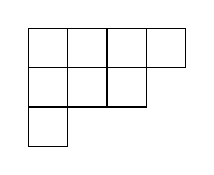
\begin{tikzpicture}[scale=0.5]
\draw (0,0) rectangle (1,1);
\draw (1,0) rectangle (2,1);
\draw (2,0) rectangle (3,1);
\draw (3,0) rectangle (4,1);
\draw (0,-1) rectangle (1,0);
\draw (1,-1) rectangle (2,0);
\draw (2,-1) rectangle (3,0);
\draw (0,-2) rectangle (1,-1);
\end{tikzpicture}
\end{center}

The column lengths of this shape form the \textcolor{blue}{conjugate partition} $\lambda'$.
In the example above, $\lambda' = (3, 2, 2, 1)$.

\end{frame}
\end{document}